\chapter{Imbalance de Clases}

Como se detalló en la sección \ref{tiles_description}, los datasets exportados por Carpyncho presentan un gran desbalance en la cantidad de estrellas etiquetadas como clase positiva (RRL) y aquellas etiquetadas con clase mayoritaria o negativa (no-RLL). En la sección \ref{imbalance} se describió, a alto nivel, qué tipo de complicaciones pueden surgir al trabajar con datasets de esta naturaleza. \\

La mayoría de los clasificadores simplemente funcionan peor en datasets desbalanceados porque están diseñádos para generalizar hallando la hipótesis más simple que se ajuste a los datos de entrenamiento, basándose en la navaja de Ockham. En datos imbalanceados, la hipótesis más simple a menudo es aquella que clasifica (casi) todas las instancias como negativas \cite{imbalanced_svm}. \\

En particular, las SVM se ven perjudicadas por el imbalance de clases \cite{imbalanced_svm}. Las instancias positivas (clase minoritaria) tienden a encontrarse más lejos de la frontera ideal \cite{wu-chang}. Esto puede ilustrarse considerando un experimento en el cuál se generan $n$ números aleatorios entre 1 y 100 a partir de una distribución uniforme. Las chances de obtener un número más cercano a 100 aumentan a mayores valores de $n$. Como consecuencia, la frontera aprendida por SVM tiende a ser más cercana a las clases positivas, tal y como se ilustra en la figura \ref{fig:skewed_svm}.\\

\begin{figure}[h!]
\centering
  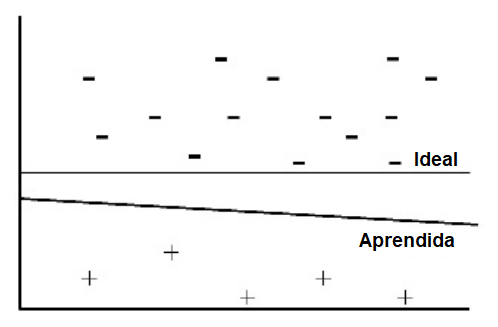
\includegraphics[width=0.45\textwidth]{Kap7/skewed_svm.png}
\caption{ Ejemplo de un dataset imbalanceado, donde las instancias positivas se encuentran más alejadas de la frontera ideal que las instancias negativas, simplemente por el hecho de ser menos. Como consecuencia, SVM aprende una frontera (línea inclinada) que está demasiado cerca de las instancias positivas. Créditos: \protect\cite{imbalanced_svm}}
\label{fig:skewed_svm}
\end{figure}

En este capítulo se experimentará con distintas técnicas que buscan atenuar el impacto del imbalance de clases, con el objeto de intentar mejorar la performance de nuestros clasificadores.

\section{Undersampling}
Las técnicas de undersampling buscan corregir manualmente el imbalance de clases en los datos, eliminando instancias de la clase mayoritaria \cite{nathalie} \cite{he}. La forma más sencilla de undersampling es \textbf{undersampling aleatorio}, en donde los elementos a descartar son elegidos aleatoriamente. Algunas consecuencias de utilizar undersampling son:

\begin{itemize}
\item Puede perderse información valiosa al descartar instancias de la clase mayoritaria.
\item La complejidad temporal y espacial para entrenar clasificadores se ve reducida, pues habrá menos datos que procesar.
\item En undersampling aleatorio, la performance del clasificador en test puede variar mucho dependiendo del sampleo utilizado.
\end{itemize}

En \cite{jbc} se experimentó utilizando undersampling aleatorio en clasificadores RF. Se concluyó que es conveniente el uso de tiles enteros, manteniendo el imbalance original entre las clases, dado que los clasificadores entrenados en tiles balanceados tenían menor performance en test. En esta sección se realizará un experimento similar utilizando SVM. \\

Se evaluó el R-AUPRC en test obtenido por clasificadores SVM entrenando con tiles artificialmente balancedas usando undersampling aleatorio, explorando distintas proporciones entre el número de no-RRLs y el número de RRLs. Nótese que cada sampleo fue obtenido del precedente, por ejemplo el sampleo con rate $1:1$ fue obtenido del sampleo con rate $1:10$ y así sucesivamente. \\

Este experimento se repitió tres veces, dado que los resultados obtenidos (especialmente para los datasets más balanceados) son sensibles al sampleo aleatorio utilizado. Los resultados para SVM lineal y SVM RBF se muestran en las figura \ref{fig:svml_undersample} y \ref{fig:svmk_undersample} respectivamente. Es importante remarcar que en todos los experimentos de este capítulo la corrección de imbalance se realiza únicamente en el tile de entrenamiento, en tanto que se usan tiles completos para testear. \\

\begin{figure}[h!]
\begin{tabular}{cccc}
  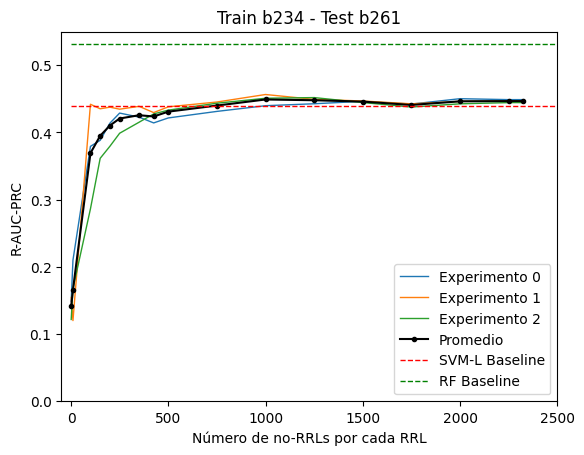
\includegraphics[width=0.25\textwidth]{Kap7/train=b234_test=b261_linear_individual_curves.png}  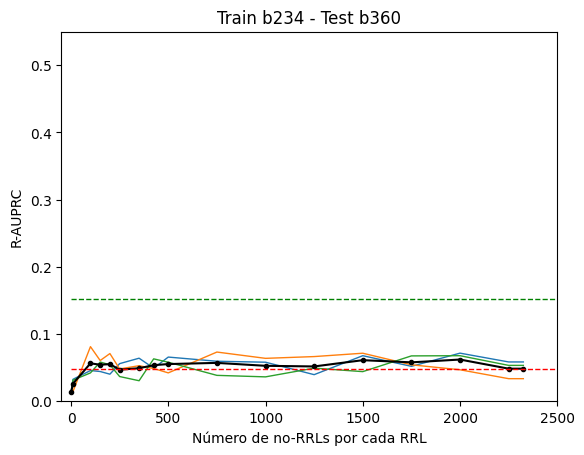
\includegraphics[width=0.25\textwidth]{Kap7/train=b234_test=b360_linear_individual_curves.png}
  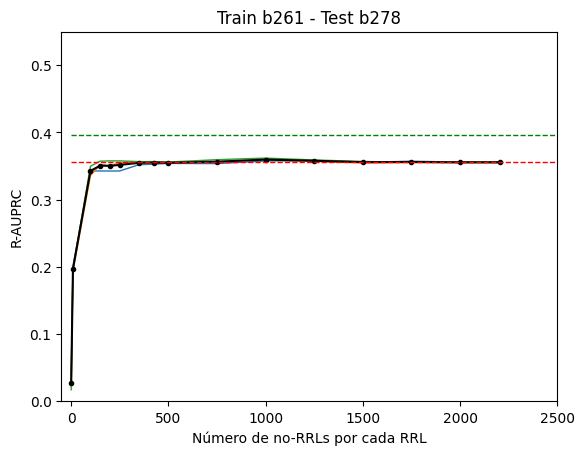
\includegraphics[width=0.25\textwidth]{Kap7/train=b261_test=b278_linear_individual_curves.png}  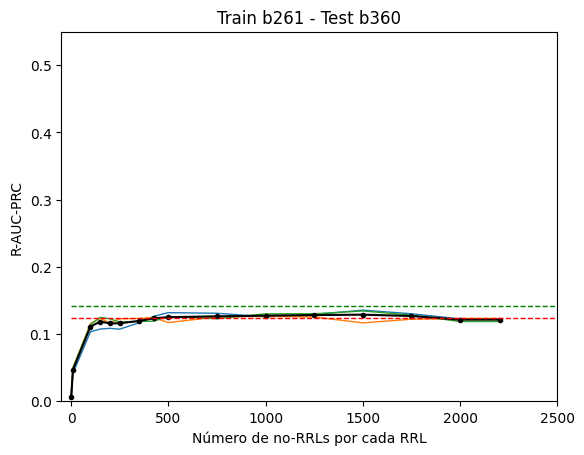
\includegraphics[width=0.25\textwidth]{Kap7/train=b261_test=b360_linear_individual_curves.png} \\

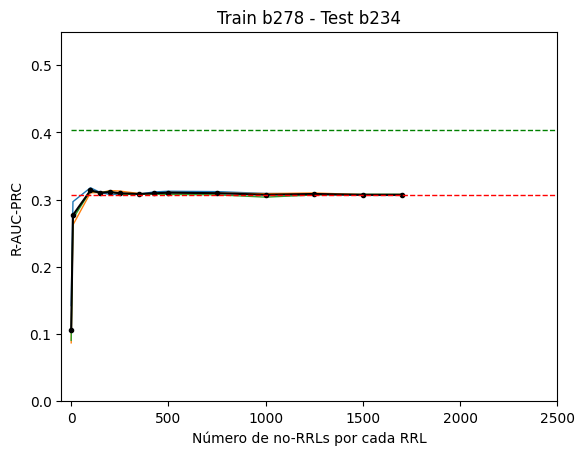
\includegraphics[width=0.25\textwidth]{Kap7/train=b278_test=b234_linear_individual_curves.png}  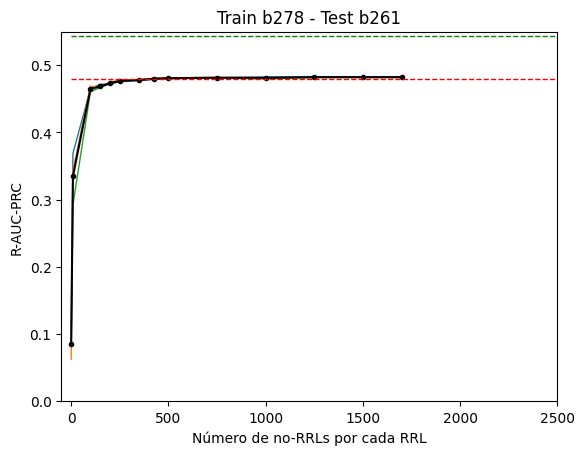
\includegraphics[width=0.25\textwidth]{Kap7/train=b278_test=b261_linear_individual_curves.png} 
 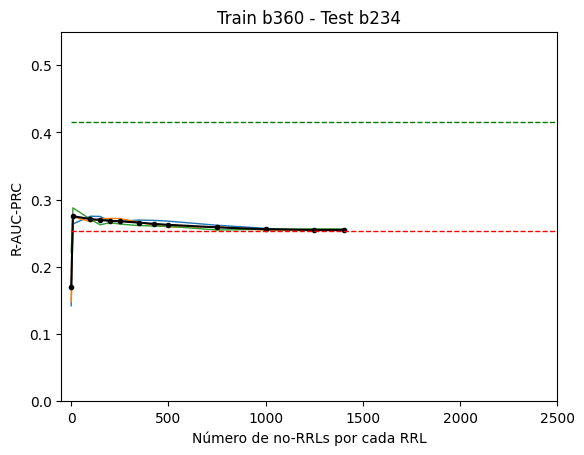
\includegraphics[width=0.25\textwidth]{Kap7/train=b360_test=b234_linear_individual_curves.png}  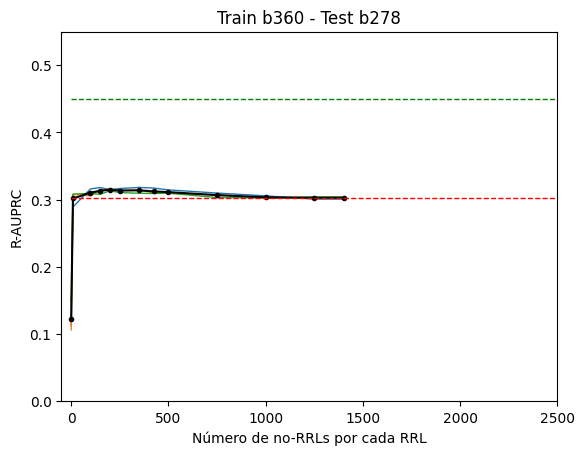
\includegraphics[width=0.25\textwidth]{Kap7/train=b360_test=b278_linear_individual_curves.png} 
\end{tabular}
\caption{Impacto de undersampling en el R-AUPRC en test de clasificadores SVM Lineal, en función de la proporción de no-RRLs por RRL. La línea punteada roja indica el R-AUPRC obtenido en la sección \protect\ref{mejores_fs}}
\label{fig:svml_undersample}
\end{figure}

\begin{figure}[h!]
\begin{tabular}{cccc}
  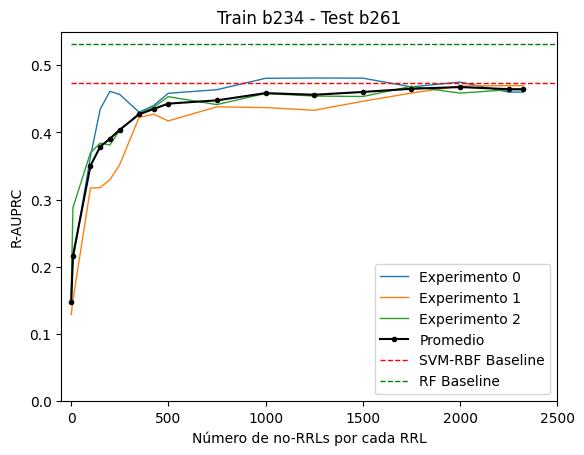
\includegraphics[width=0.25\textwidth]{Kap7/train=b234_test=b261_rbf_individual_curves.png}  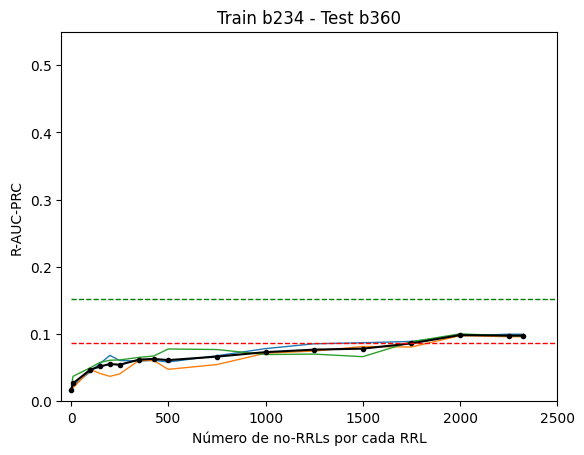
\includegraphics[width=0.25\textwidth]{Kap7/train=b234_test=b360_rbf_individual_curves.png}
  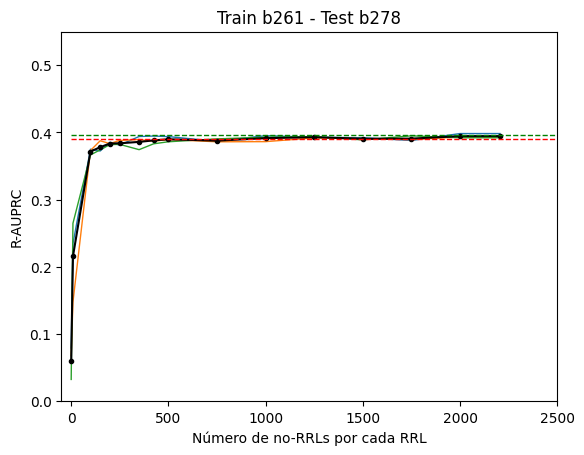
\includegraphics[width=0.25\textwidth]{Kap7/train=b261_test=b278_rbf_individual_curves.png}  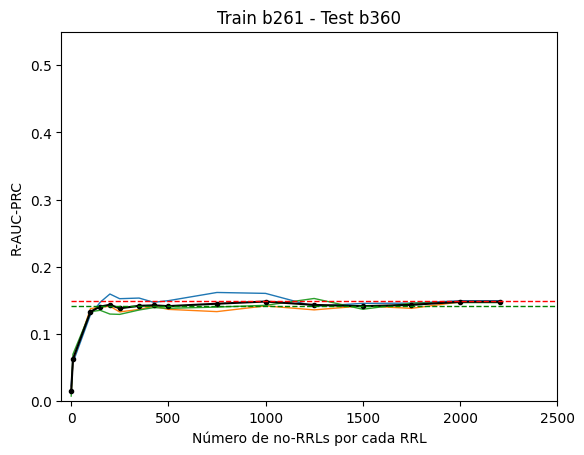
\includegraphics[width=0.25\textwidth]{Kap7/train=b261_test=b360_rbf_individual_curves.png} \\

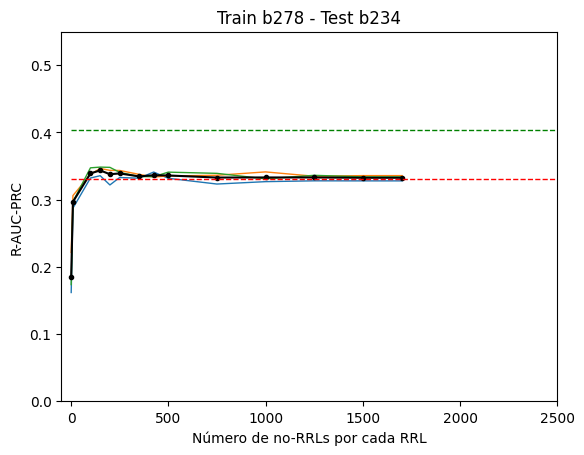
\includegraphics[width=0.25\textwidth]{Kap7/train=b278_test=b234_rbf_individual_curves.png}  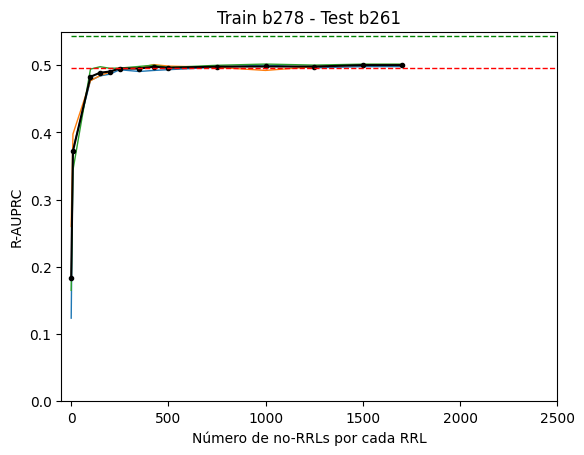
\includegraphics[width=0.25\textwidth]{Kap7/train=b278_test=b261_rbf_individual_curves.png} 
 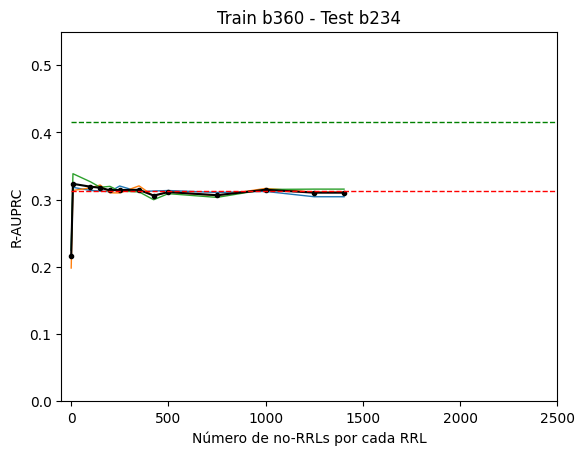
\includegraphics[width=0.25\textwidth]{Kap7/train=b360_test=b234_rbf_individual_curves.png}  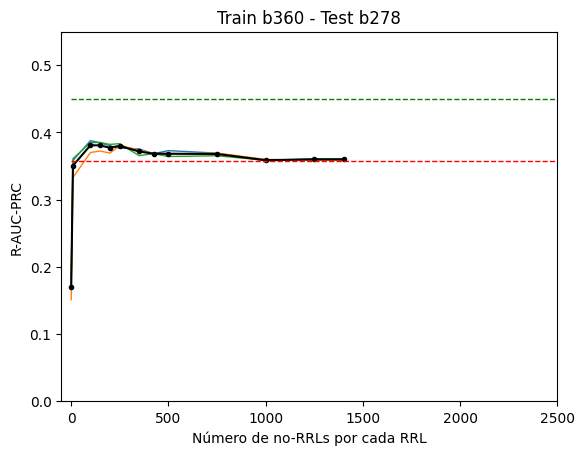
\includegraphics[width=0.25\textwidth]{Kap7/train=b360_test=b278_rbf_individual_curves.png} 
\end{tabular}
\caption{Impacto de undersampling en el R-AUPRC en test de clasificadores SVM RBF, en función de la proporción de no-RRLs por RRL. La línea punteada roja indica el R-AUPRC obtenido en la sección \protect\ref{mejores_fs}}
\label{fig:svmk_undersample}
\end{figure}

Utilizando las curvas de color negro, se calculó la ganancia promedio (entre todos los tiles) en R-AUPRC respecto al baseline, para cada proporción RRL-noRRL estudiada. Los resultados de estos experimentos se encuentran en la figura \ref{fig:overall_undersampling}, de los cuáles podemos concluir:
\begin{itemize}
\item Balancear las clases en exceso es altamente perjudicial, pues reduce el R-AUPRC drásticamente para todos los tiles (ver las curvas en proporciones 1:1 a 1:250).
\item En SVM Lineal, corregir el imbalance de forma moderada, dejando al menos 500 no-RRL por RRL, permite igualar el baseline. Esto implica que se puede obtener al menos la misma performance en test utilizando tan solo un cuarto datos para entrenar. Una consecuencia inmediata es una drástica reducción en la complejidad temporal y espacial necesaria para entrenar clasificadores SVM Lineal.
\item En SVM-RBF, undersampling incurre en una pérdida de R-AUPRC promedio para todas las proporciones testeadas.
\end{itemize}

Undersampling resulta, por lo tanto, no útil para mejorar el R-AUPRC de nuestros clasificadores. Únicamente resulta beneficioso en SVM Lineal, para obtener una reducción importante en tiempos de entrenamiento y consumo de memoria.

\begin{figure}[h!]
\begin{tabular}{cc}
  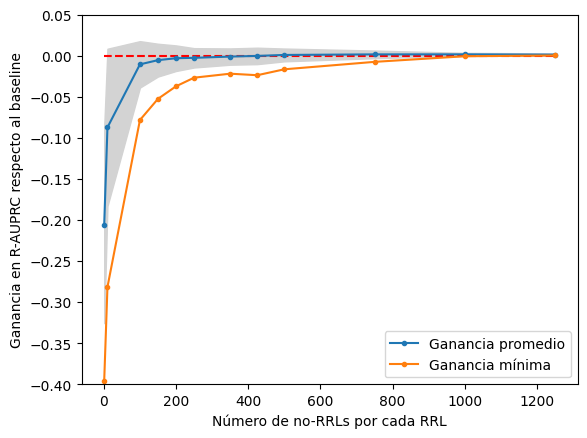
\includegraphics[width=0.49\textwidth]{Kap7/linearBEST.png} &   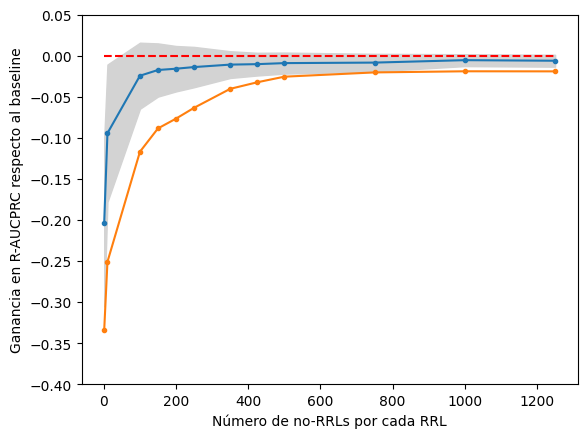
\includegraphics[width=0.49\textwidth]{Kap7/rbfBEST.png} \\
(a) SVM Lineal& (b) SVM RBF
\end{tabular}
\caption{ Ganancia promedio en R-AUPRC respecto al baseline al utilizar undersampling, en función de la proporción entre las clases. Nótese que el dominio de estos gráficos se extiende sólo hasta 1200, pues es la proporción original de algunos de los tiles estudiados. La mayoría de los tiles, sin embargo, presenta un imbalance original de 1:2000. }
\label{fig:overall_undersampling}
\end{figure}

\section{Oversampling}

Una segunda forma de corregir manualmente el imbalance de las clases consiste en generar nuevas instancias de la clase minoritaria \cite{he}. En este trabajo se usaron tres métodos para lograr esto, ilustrados en la figura \ref{fig:oversampling_comparison}:

\begin{itemize}
\item \textbf{Oversampling aleatorio}: Seleccionar elementos de la clase minoritaria (con reemplazo) con probabilidad uniforme, añadiéndolos nuevamente al dataset de entrenamiento \cite{Menardi2012TrainingAA}. Como consecuencia, habrá instancias repetidas.
\item \textbf{ADASYN} (Adaptative Synthetic sampling method): Generar nuevas instancias utilizando interpolación, intentando crear puntos cerca de aquellas instancias que son incorrectamente clasificadas utilizando kNN.\cite{adasyn}
\item \textbf{SMOTE} (Synthetic Minority Oversampling Technique): Generar nuevas instancias utilizando interpolación, sin hacer ninguna distinción entre instancias que son fáciles o difíciles de clasificar. \cite{smote}
\end{itemize}

Adicionalmente, se experimentó con una técnica híbrida que combina undersampling y oversampling:
\begin{itemize}
\item \textbf{SMOTEENN}: Consiste en generar nuevas instancias utilizando SMOTE, seguido de una eliminación de instancias ruidosas utilizando el método de undersampling ENN (Edited Nearest Neighbors) \cite{Batista2003BalancingTD}. Podemos ver un ejemplo de SMOTEENN en la figura \ref{fig:smoteenn}.
\end{itemize}

\begin{figure}[h!]
\centering
  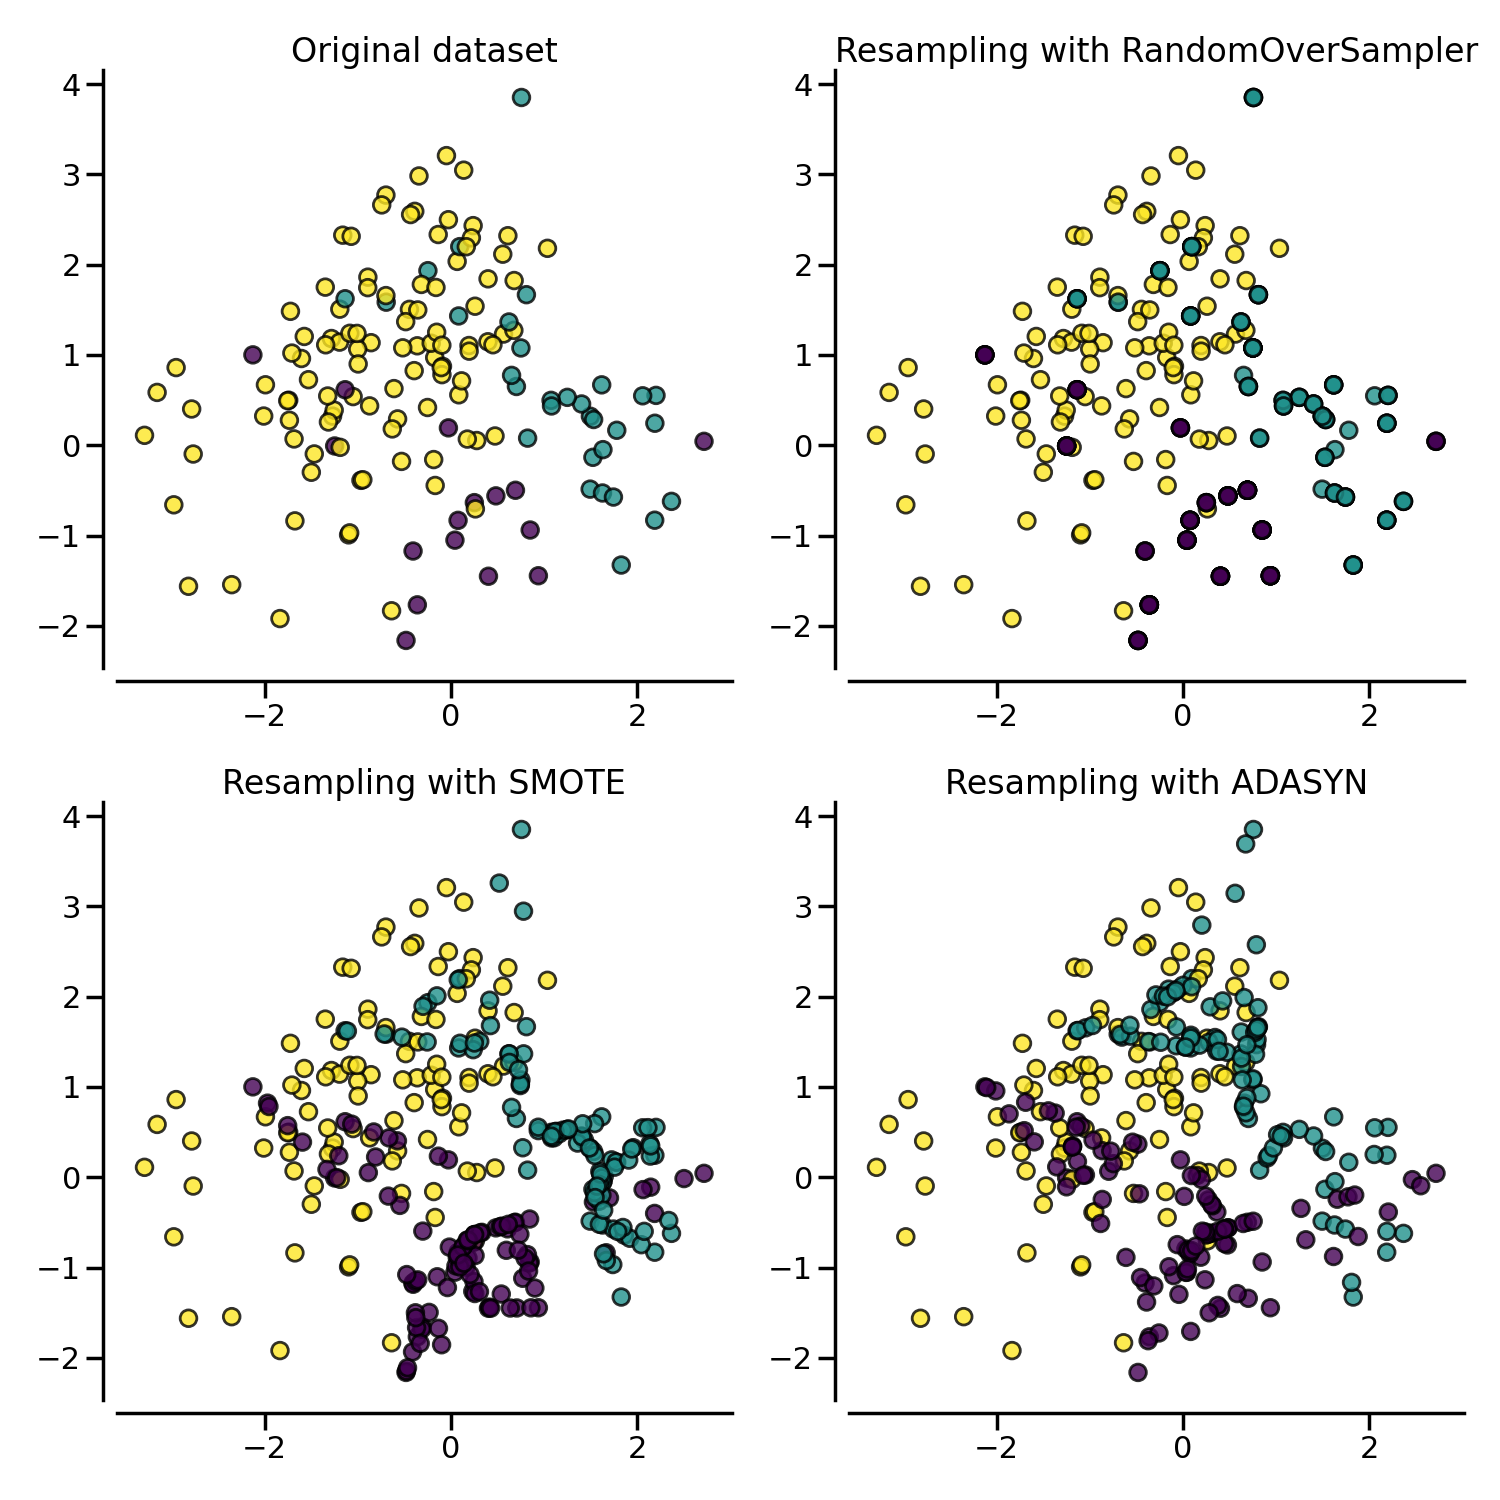
\includegraphics[width=0.9\textwidth]{Kap7/oversampling_comparison.png}
\caption{ Comparación de métodos de oversampling utilizados en este trabajo. Créditos: Documentación de \textit{imbalanced-learn}.}
\label{fig:oversampling_comparison}
\end{figure}

\begin{figure}[h!]
\begin{tabular}{ccc}
  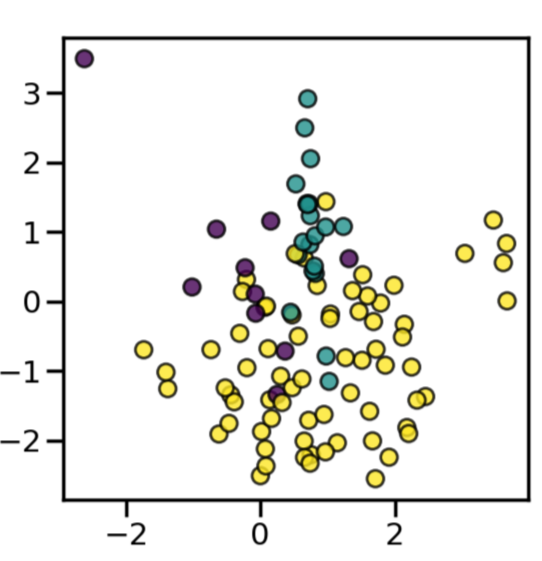
\includegraphics[width=0.32\textwidth]{Kap7/smoteenn_1.png} & 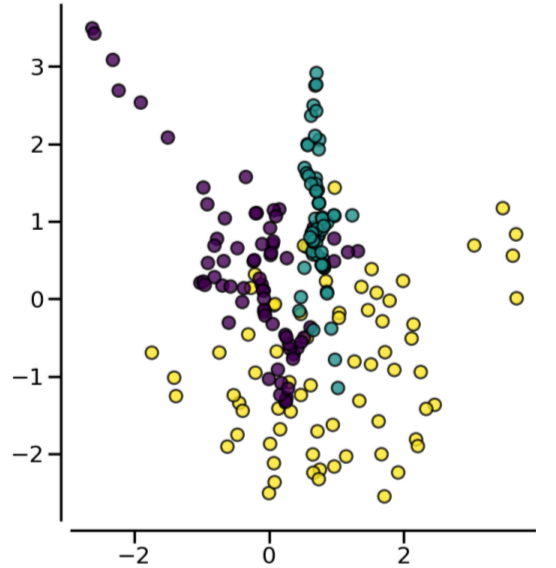
\includegraphics[width=0.32\textwidth]{Kap7/smoteenn_2.png} & 
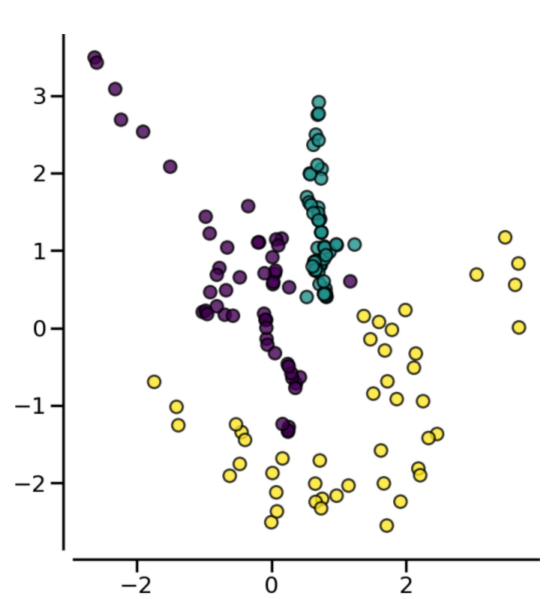
\includegraphics[width=0.32\textwidth]{Kap7/smoteenn_3.png} \\
(a) Datos originales & (b) Oversampling SMOTE & (c) SMOTEENN
\end{tabular}
\caption{ Aplicación de SMOTEENN sobre el dataset imbalanceado (a). En primer lugar, se aplica oversampling SMOTE (b). Finalmente, se eliminan algunas de las nuevas instancias utilizando ENN (c). Créditos: Documentación de \textit{imbalanced-learn}. }
\label{fig:smoteenn}
\end{figure}


Se utilizaron las implementaciones provistas por \textbf{imbalanced-learn} (\url{imbalanced-learn.org/}), una librería que extiende scikit-learn con técnicas para abordar imbalance de clases. De forma similar a la sección anterior, se analizó el impacto en R-AUPRC en función a la proporción de RRLs y no-RRLs para cada método estudiado. Los resultados de este experimento para SVM Lineal y SVM RBF se encuentran en las figuras \ref{fig:svm_oversampling} y \ref{fig:svmk_oversampling} respectivamente.\\

\begin{figure}[h!]
\begin{tabular}{cccc}

  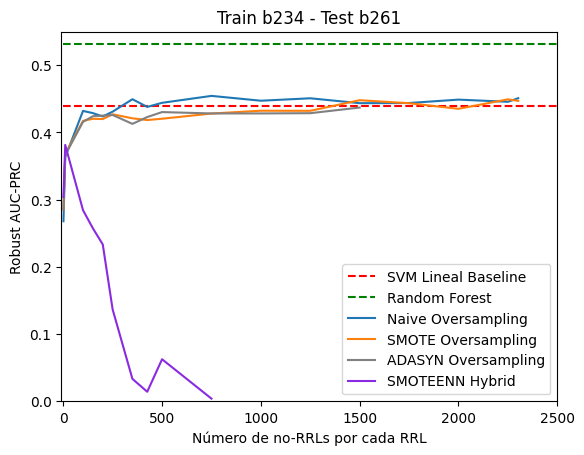
\includegraphics[width=0.25\textwidth]{Kap7/UNIFIED_train=b234_test=b261_linear_curves.png}  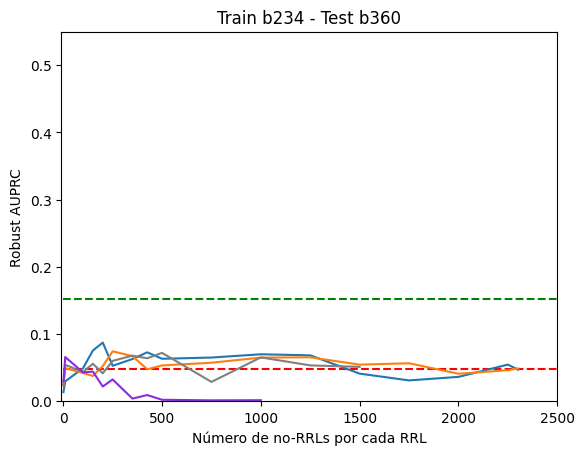
\includegraphics[width=0.25\textwidth]{Kap7/UNIFIED_train=b234_test=b360_linear_curves.png}
  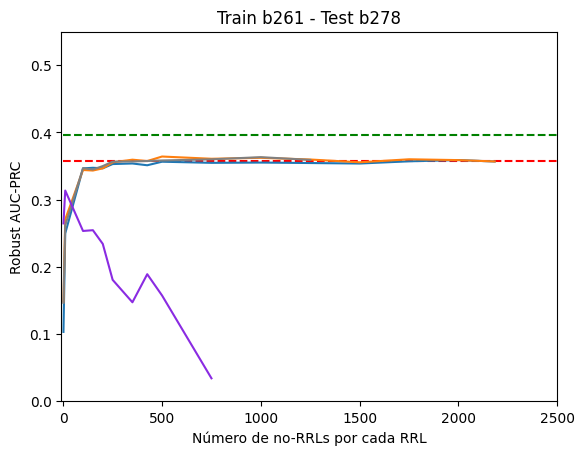
\includegraphics[width=0.25\textwidth]{Kap7/UNIFIED_train=b261_test=b278_linear_curves.png}  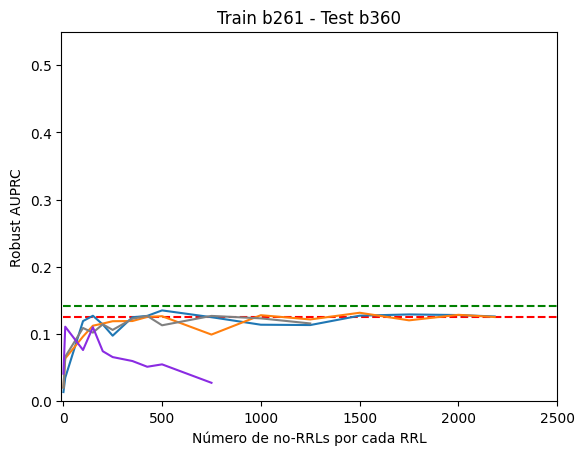
\includegraphics[width=0.25\textwidth]{Kap7/UNIFIED_train=b261_test=b360_linear_curves.png} \\

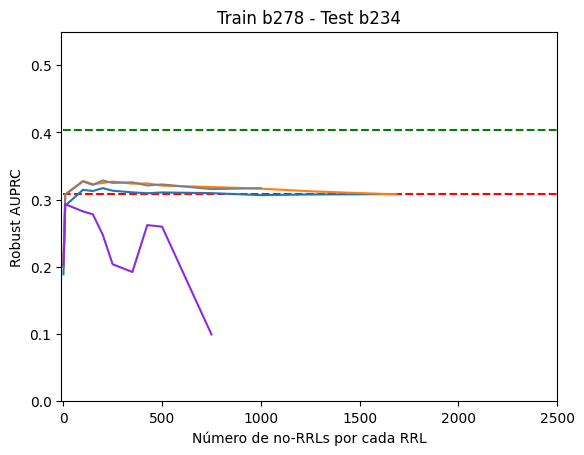
\includegraphics[width=0.25\textwidth]{Kap7/UNIFIED_train=b278_test=b234_linear_curves.png}  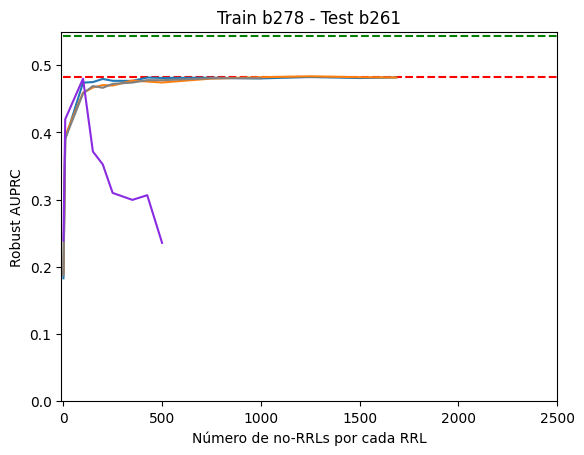
\includegraphics[width=0.25\textwidth]{Kap7/UNIFIED_train=b278_test=b261_linear_curves.png} 
 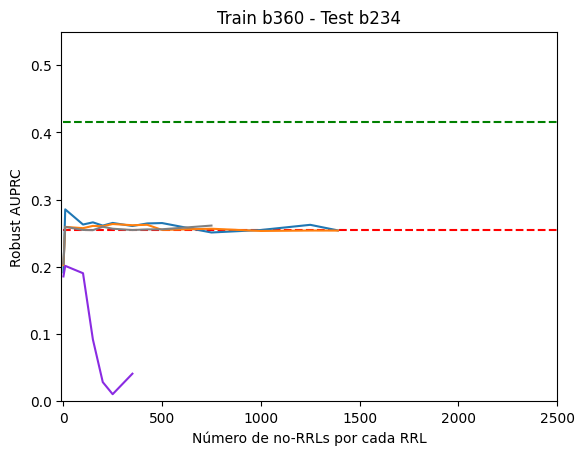
\includegraphics[width=0.25\textwidth]{Kap7/UNIFIED_train=b360_test=b234_linear_curves.png}  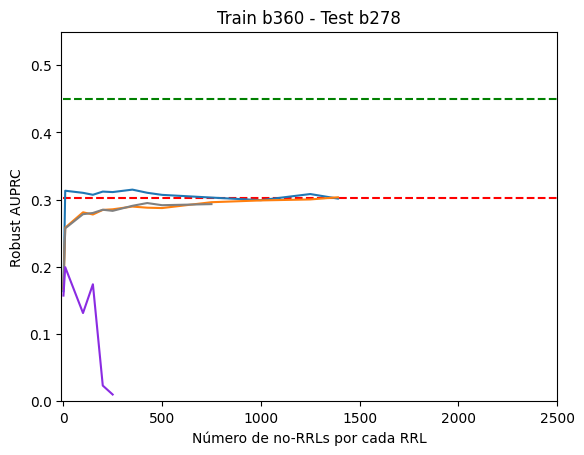
\includegraphics[width=0.25\textwidth]{Kap7/UNIFIED_train=b360_test=b278_linear_curves.png} 
\end{tabular}
\caption{Impacto de oversampling en el R-AUPRC en test de clasificadores SVM Lineal, en función de la proporción de no-RRLs por RRL. La línea punteada roja indica el R-AUPRC obtenido en la sección \protect\ref{mejores_fs}}
\label{fig:svm_oversampling}
\end{figure}

\begin{figure}[h!]
\begin{tabular}{cccc}

  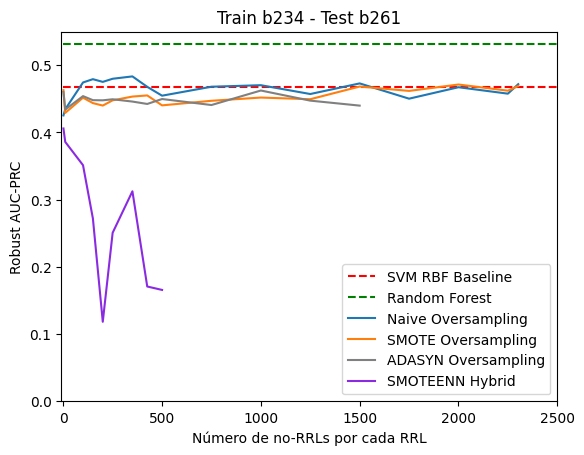
\includegraphics[width=0.25\textwidth]{Kap7/UNIFIED_train=b234_test=b261_rbf_curves.png}  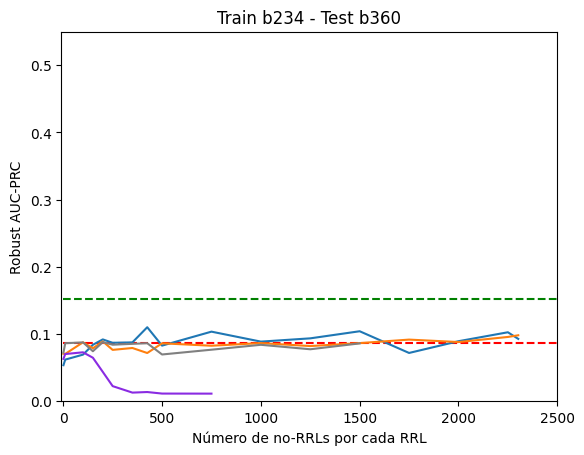
\includegraphics[width=0.25\textwidth]{Kap7/UNIFIED_train=b234_test=b360_rbf_curves.png}
  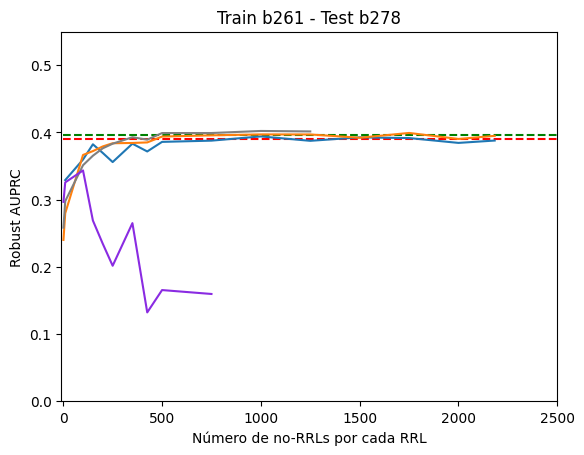
\includegraphics[width=0.25\textwidth]{Kap7/UNIFIED_train=b261_test=b278_rbf_curves.png}  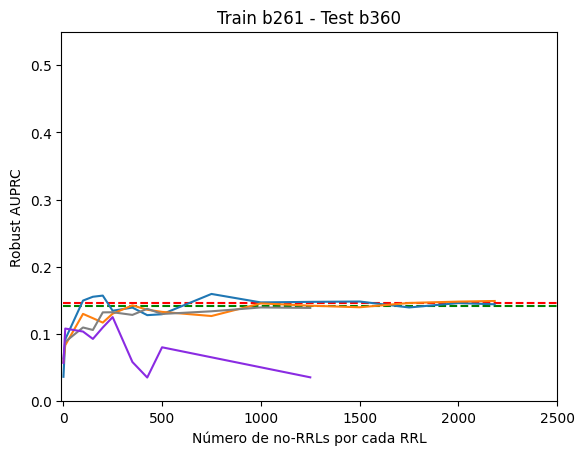
\includegraphics[width=0.25\textwidth]{Kap7/UNIFIED_train=b261_test=b360_rbf_curves.png} \\

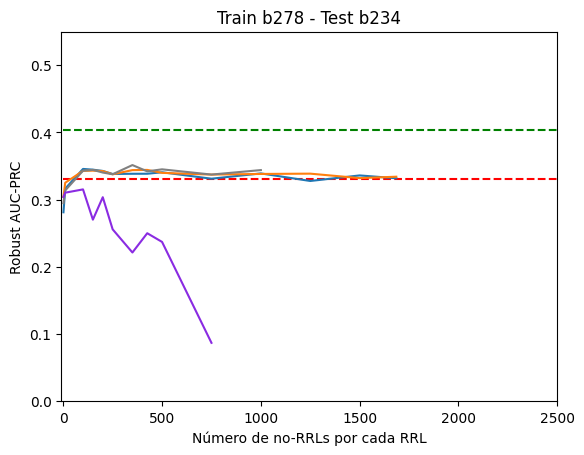
\includegraphics[width=0.25\textwidth]{Kap7/UNIFIED_train=b278_test=b234_rbf_curves.png}  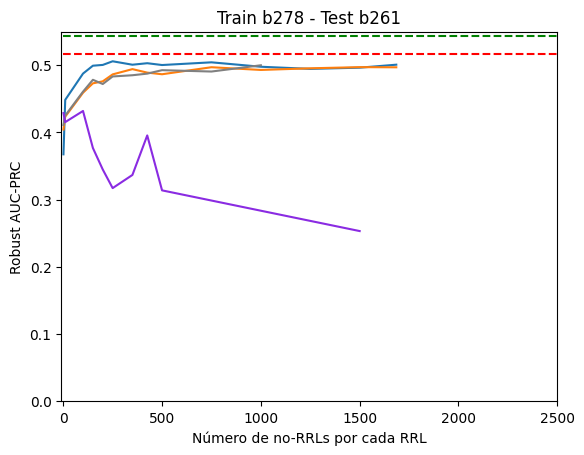
\includegraphics[width=0.25\textwidth]{Kap7/UNIFIED_train=b278_test=b261_rbf_curves.png} 
 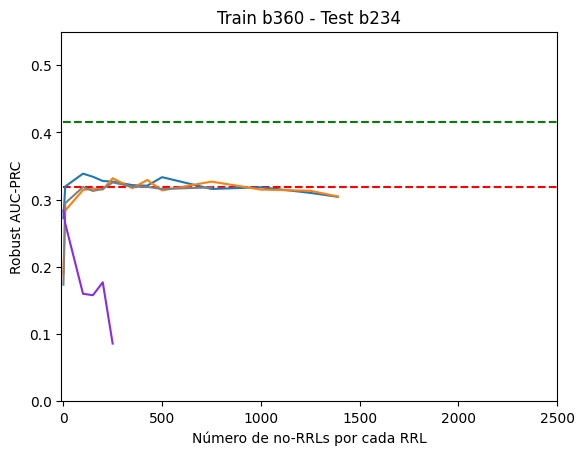
\includegraphics[width=0.25\textwidth]{Kap7/UNIFIED_train=b360_test=b234_rbf_curves.png}  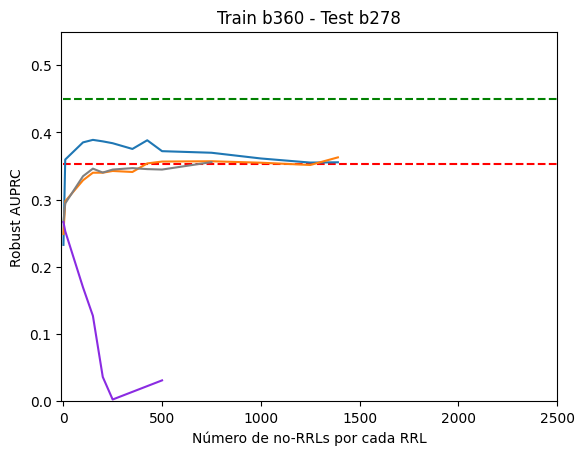
\includegraphics[width=0.25\textwidth]{Kap7/UNIFIED_train=b360_test=b278_rbf_curves.png} 
\end{tabular}
\caption{Impacto de oversampling en el R-AUPRC en test de clasificadores SVM RBF, en función de la proporción de no-RRLs por RRL. La línea punteada roja indica el R-AUPRC obtenido en la sección \protect\ref{mejores_fs}}
\label{fig:svmk_oversampling}
\end{figure}

En primer lugar, podemos descartar el método SMOTEENN como preprocesamiento de nuestros tiles, debido a su pobre performance en todos los casos evaluados. Para los tres métodos restantes, se calcularon las ganancias promedio respecto al baseline, las cuales se encuentran graficadas en la figura \ref{fig:overall_oversampling} . Podemos concluír que:
\begin{itemize}
\item En SVM Lineal, únicamente oversampling aleatorio es capaz de mejorar levemente el R-AUPRC baseline en promedio. No hay beneficio en aplicar ADASYN o SMOTE.
\item Similarmente, en SVM RBF, ADASYN y SMOTE empeoran el R-AUPRC respecto al baseline en promedio. Oversampling aleatorio, en el mejor caso, logra igualar o superar el R-AUPRC promedio pero con una pérdida importante en el peor caso.
\item Notar que, al igual que en undersampling, corregir el imbalance en exceso (500 o menos no-RRl por RRL) incurre en una reducción notable en R-AUPRC.
\item Es importante notar que al hacer oversampling, una corrección moderada del imbalance (con 500 o más no-RRL por RRL) implica un aumento importante en el tamaño de los datasets de entrenamiento. Esto conlleva un mayor consumo de memoria y tiempo de entrenamiento.
\end{itemize}

\begin{figure}[h!]
\begin{tabular}{cc}
  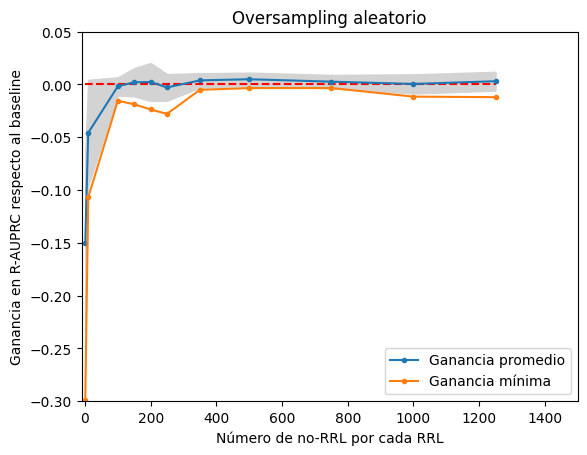
\includegraphics[width=0.49\textwidth]{Kap7/aleatorio_linearBEST.png} & 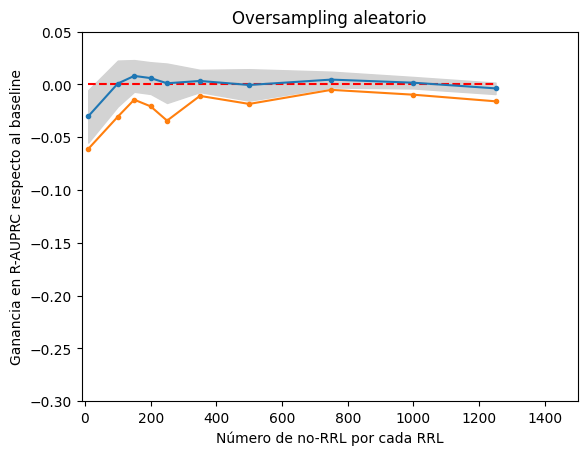
\includegraphics[width=0.49\textwidth]{Kap7/aleatorio_rbfBEST.png} \\
   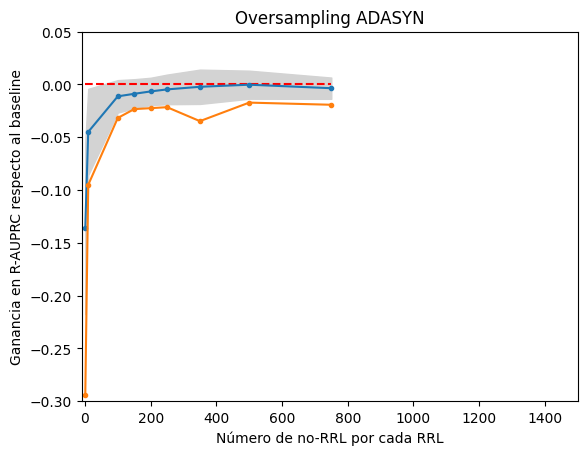
\includegraphics[width=0.49\textwidth]{Kap7/ADASYN_linearBEST.png} & 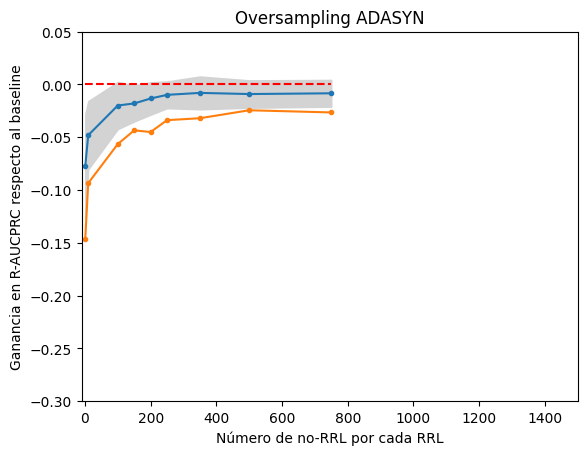
\includegraphics[width=0.49\textwidth]{Kap7/ADASYN_rbfBEST.png} \\
    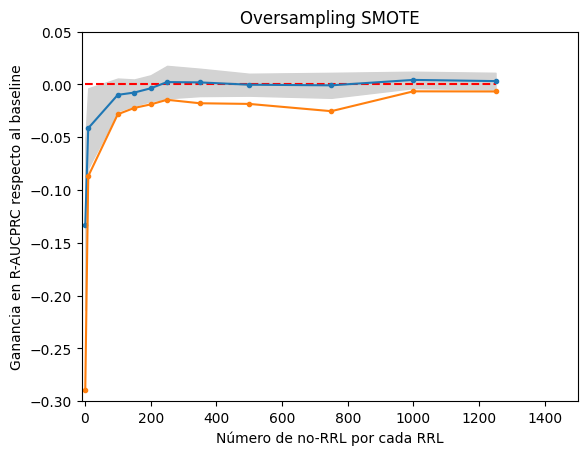
\includegraphics[width=0.49\textwidth]{Kap7/SMOTE_linearBEST.png} & 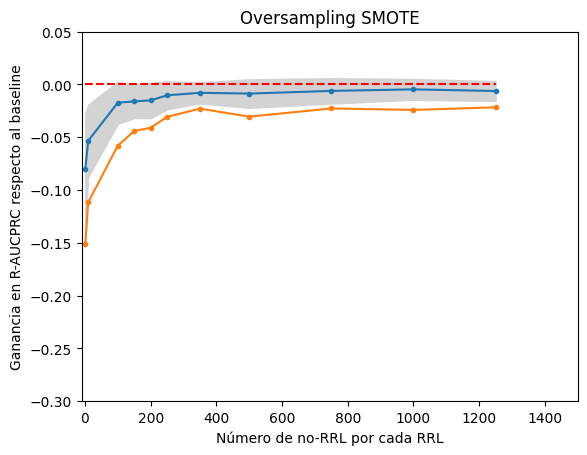
\includegraphics[width=0.49\textwidth]{Kap7/SMOTE_rbfBEST.png} \\
(a) SVM Lineal& (b) SVM RBF
\end{tabular}
\caption{ Ganancia promedio en R-AUPRC respecto al baseline al utilizar oversampling, en función de la proporción entre las clases }
\label{fig:overall_oversampling}
\end{figure}

En resumen, los resultados son similares a los vistos para undersampling: Oversampling no es beneficioso en SVM RBF, y es ligeramente beneficioso para SVM-Lineal. Sin embargo, esta mejoría en R-AUPRC conlleva un mayor costo de procesamiento y memoria. 

\section{Class Weight}

Un tercer enfoque orientado a resolver el efecto del imbalance de clases es sesgar el clasificador de forma tal que preste más atención a la clase positiva \cite{imbalanced_svm}. Esto puede hacerse, por ejemplo, incrementando la penalidad asociada a clasificar incorrectamente las instancias de clase RRL. \\

La implementación de SVM provista por sklearn permite asignar un peso $\alpha_i$ a cada clase $i$, de forma tal que se penalicen los errores de cada clase con una severidad diferente, ajustando el parámetro de regularización $C$ como $\alpha_i * C$ para cada clase $i$ . En problemas de clasificación binaria, llamaremos $\alpha_+$ y $\alpha_-$ a los pesos de la clase minoritaria (positiva) y mayoritaria (negativa), respectivamente. \\

Se evaluó el impacto en R-AUPRC en test obtenido al utilizar SVM con distintos valores de $\alpha_{+}$, fijando $\alpha_{-}=1$. Los resultados para SVM Lineal y SVM RBF se encuentran en las figuras \ref{fig:cw_l} y \ref{fig:cw_k} respectivamente. \\

\begin{figure}[h!]
\begin{tabular}{cccc}
  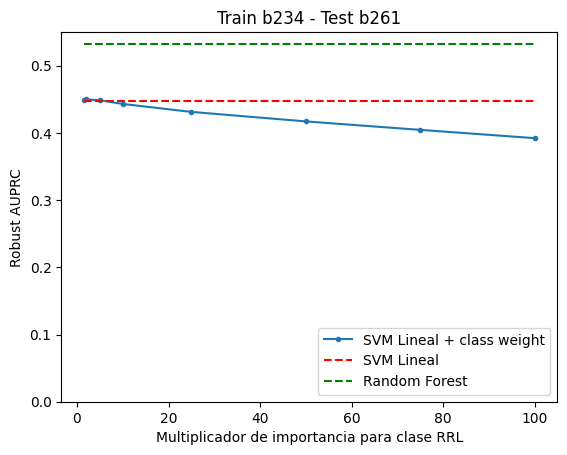
\includegraphics[width=0.25\textwidth]{Kap7/cw/train=b234_test=b261_linear_individual_curves.png}  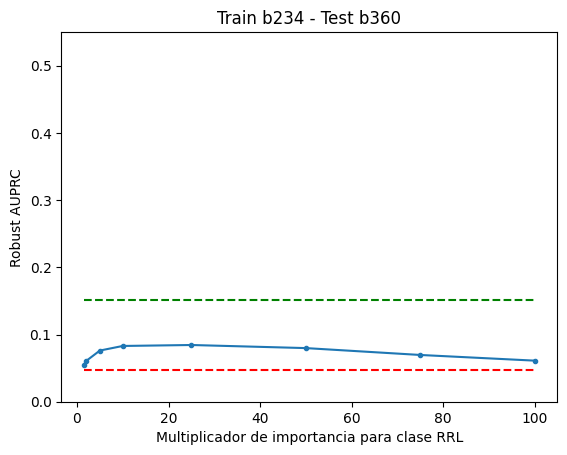
\includegraphics[width=0.25\textwidth]{Kap7/cw/train=b234_test=b360_linear_individual_curves.png}
  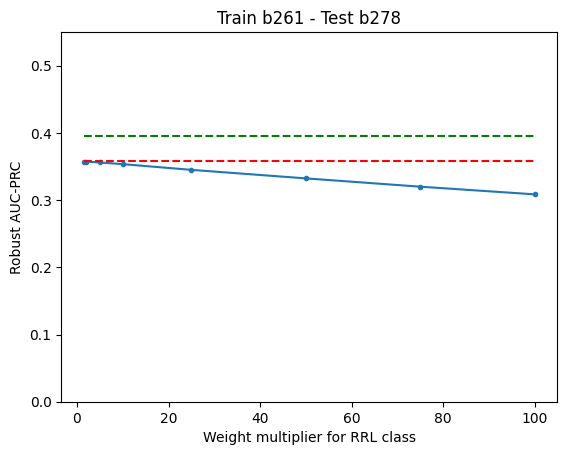
\includegraphics[width=0.25\textwidth]{Kap7/cw/train=b261_test=b278_linear_individual_curves.png}  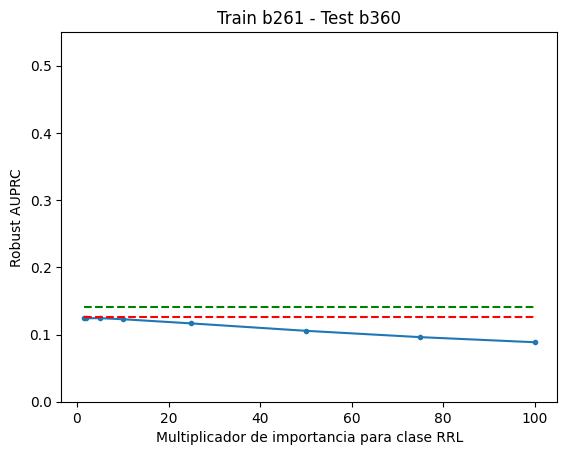
\includegraphics[width=0.25\textwidth]{Kap7/cw/train=b261_test=b360_linear_individual_curves.png} \\

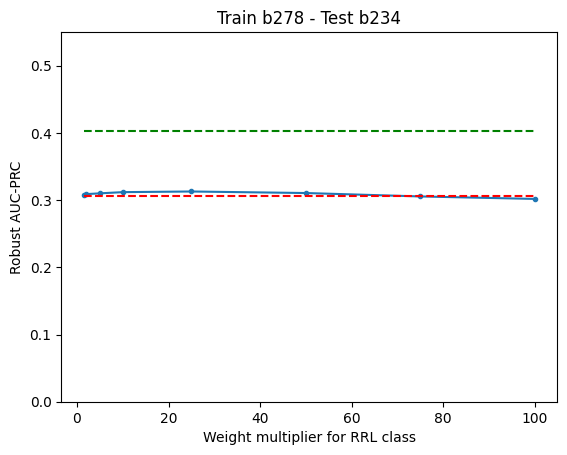
\includegraphics[width=0.25\textwidth]{Kap7/cw/train=b278_test=b234_linear_individual_curves.png}  \includegraphics[width=0.25\textwidth]{Kap7/cw/train=b278_test=b261_linear_individual_curves.png} 
 \includegraphics[width=0.25\textwidth]{Kap7/cw/train=b360_test=b234_linear_individual_curves.png}  \includegraphics[width=0.25\textwidth]{Kap7/cw/train=b360_test=b278_linear_individual_curves.png} 
\end{tabular}
\caption{Impacto de class weight en el R-AUPRC en test de clasificadores SVM Lineal, en función del multiplicador a la penalidad de la clase positiva. La línea punteada roja indica el R-AUPRC obtenido en la sección \protect\ref{mejores_fs}}
\label{fig:cw_l}
\end{figure}

\begin{figure}[h!]
\begin{tabular}{cccc}
  \includegraphics[width=0.25\textwidth]{Kap7/cw/train=b234_test=b261_rbf_individual_curves.png}  \includegraphics[width=0.25\textwidth]{Kap7/cw/train=b234_test=b360_rbf_individual_curves.png}
  \includegraphics[width=0.25\textwidth]{Kap7/cw/train=b261_test=b278_rbf_individual_curves.png}  \includegraphics[width=0.25\textwidth]{Kap7/cw/train=b261_test=b360_rbf_individual_curves.png} \\

\includegraphics[width=0.25\textwidth]{Kap7/cw/train=b278_test=b234_rbf_individual_curves.png}  \includegraphics[width=0.25\textwidth]{Kap7/cw/train=b278_test=b261_rbf_individual_curves.png} 
 \includegraphics[width=0.25\textwidth]{Kap7/cw/train=b360_test=b234_rbf_individual_curves.png}  \includegraphics[width=0.25\textwidth]{Kap7/cw/train=b360_test=b278_rbf_individual_curves.png} 
\end{tabular}
\caption{Impacto de class weight en el R-AUPRC en test de clasificadores SVM RBF, en función del multiplicador a la penalidad de la clase positiva. La línea punteada roja indica el R-AUPRC obtenido en la sección \protect\ref{mejores_fs}}
\label{fig:cw_k}
\end{figure}

Si bien el uso de $class\_weight$ tiene un impacto  positivo en algunos pares de tiles; tiene un impacto igualmente perjudicial en otros pares. La figura \ref{fig:overall_cw} resume esta información, permitiéndonos concluir que:

\begin{itemize}
\item $class\_weight$ permite obtener una mejora promedio leve en SVM-Lineal para $ 1 < \alpha_+ < 20$, y una mejora promedio casi nula en SVM-RBF para $1 < \alpha_+ < 10$.
\item La mejoría promedio viene acompañada de reducción marcada en R-AUPRC para algunos pares de tiles. Esto indica que el uso de $class\_weight$ produce resultados un tanto inestables.
\end{itemize}

\begin{figure}[h!]
\begin{tabular}{cc}
  \includegraphics[width=0.49\textwidth]{Kap7/cw/linearBEST.png} &   \includegraphics[width=0.49\textwidth]{Kap7/cw/rbfBEST.png} \\
(a) SVM Lineal& (b) SVM RBF
\end{tabular}
\caption{ Ganancia promedio en R-AUPRC respecto al baseline al utilizar class weight, en función del multiplicador a la penalidad de la clase positiva.  }
\label{fig:overall_cw}
\end{figure}

\section{Conclusiones}
\label{conclusion_imb}

Con el objeto de mitigar el impacto del imbalance de clases, en este capítulo se hizo uso de técnicas de oversampling y undersampling. También se intento sesgar los clasificadores SVM para que presten más atención a la clase minoritaria. Ninguna de las técnicas estudiadas logró mejorar significativamente el R-AUPRC baseline obtenido en capítulos anteriores. \\

Continuando con la política establecida en capítulos anteriores, se preferirá aquél preprocesamiento que maximice la ganancia promedio en R-AUPRC sujeto a no empeorar significativamente el R-AUPRC en ningún par de tiles estudiados. Esta última condición busca prevenir métodos con resultados inestables, que son altamente dependientes del par de tiles elegido. \\

Los hiperparámetros que maximizan esta métrica para SVM Lineal se muestran en la tabla \ref{tab:best_hyp_svml}. Por otro lado, en SVM RBF, si bien algunos métodos logran mejorar el R-AUPRC promedio muy ligeramente, la ganancia mínima para algunos pares es demasiado negativa. Los resultados para SVM RBF se encuentran en la tabla \ref{tab:best_hyp_svmk}. 


\begin{table}[ht]
\centering
\begin{tabular}{c|c|c|c|}
\cline{2-4}
\textbf{}                                             & \textbf{Hiperparámetro óptimo} & \textbf{Avg gain} & \textbf{Min gain} \\ \hline
\multicolumn{1}{|c|}{\textbf{Undersampling aletorio}} & Proporción: 1:1000       & 0.004             & 0.001            \\ \hline
\multicolumn{1}{|c|}{\textbf{Oversampling aleatorio}} & Proporción: 1:500        & 0.007             & -0.001            \\ \hline
\multicolumn{1}{|c|}{\textbf{Class weight}}           & $\alpha_+$ = 2           & 0.005             & 0            \\ \hline
\end{tabular}
\caption{Hiperparámetros óptimos para los mejores métodos estudiados en esta sección, SVM-L. El criterio de optimalidad es: maximizar la ganancia promedio respecto al baseline, sujeto a no empeorar la performance en ningún par de tiles significativamente.}
\label{tab:best_hyp_svml}
\end{table}

 
\begin{table}[ht]
\centering
\begin{tabular}{c|c|c|c|}
\cline{2-4}
\textbf{}                                             & \textbf{Hiperparámetro óptimo} & \textbf{Avg gain} & \textbf{Min gain} \\ \hline
\multicolumn{1}{|c|}{\textbf{Undersampling aletorio}} &  $\nexists$       &  -       &  - \\ \hline
\multicolumn{1}{|c|}{\textbf{Oversampling aleatorio}} & Proporción: 1:750        &  0.003       & -0.013 \\ \hline
\multicolumn{1}{|c|}{\textbf{Class weight}}           & $\alpha_+$ = 5    & 0.006     & -0.015             \\ \hline
\end{tabular}
\caption{Hiperparámetros óptimos para los mejores métodos estudiados en esta sección, SVM-RBF. Dado que no existen hiperparámetros que no empeoren la performance en ningún par de tiles significativamente, se muestran los hiperparámetros que maximizan la ganancia mínima. }
\label{tab:best_hyp_svmk}
\end{table}

Se decidió elegir oversampling aleatorio con proporción 1:500 como preprocesamiento para SVM Lineal en el resto de este trabajo, aunque la mejoría es casi nula. En la tabla \ref{tab:imb_comparison_l} se muestra la mejora obtenida para una selección de tiles. Para SVM-RBF, todos los métodos estudiados empeoran significativamente el R-AUPRC en alguno de los tiles estudiados, a cambio de una ganancia casi nula en promedio; por lo que se decidió no realizar corrección de imbalance alguna. \\

Como conclusión de este capítulo, podemos decir que el imbalance de clases parece no estar teniendo un impacto tan perjudicial en SVM, pues las técnicas de corrección de imbalance no permiten mejorar resultados significativamente.

\begin{table}[ht]
\centering
\begin{tabular}{|c|c|c|c|c|c|}
\hline
\textbf{Train tile} & \textbf{Test tile} & \textbf{RF} & \textbf{SVM-L sin overs.} & \textbf{SVM-L con overs.} & \textbf{Gain} \\ \hline
b278                & b234               & 0.40        & 0.307                     & 0.312                     & 0.005         \\ \hline
b278                & b261               & 0.54        & 0.479                     & 0.48                      & 0.001         \\ \hline
b278                & b360               & 0.21        & 0.134                     & 0.135                     & 0.001         \\ \hline
b234                & b278               & 0.40        & 0.305                     & 0.313                     & 0.009         \\ \hline
b234                & b261               & 0.53        & 0.439                     & 0.45                      & 0.011         \\ \hline
b234                & b360               & 0.15        & 0.044                     & 0.057                     & 0.014         \\ \hline
b261                & b278               & 0.40        & 0.358                     & 0.355                     & -0.003        \\ \hline
b261                & b234               & 0.39        & 0.3                       & 0.301                     & 0.001         \\ \hline
b261                & b360               & 0.14        & 0.125                     & 0.135                     & 0.01          \\ \hline
b360                & b278               & 0.45        & 0.3                       & 0.307                     & 0.007         \\ \hline
b360                & b234               & 0.42        & 0.253                     & 0.26                      & 0.007         \\ \hline
b360                & b261               & 0.54        & 0.406                     & 0.414                     & 0.007         \\ \hline
\multicolumn{2}{|c|}{AVG}                & 0.38        & 0.287                     & 0.293                     & 0.005         \\ \hline
\end{tabular}
\caption{En esta tabla podemos ver el incremento en R-AUPRC que se obtiene al utilizar oversampling 1:500 en SVM-Lineal. }
\label{tab:imb_comparison_l} 
\end{table}
